



\part{Background}
\label{part:background}

%======================================================================
\chapter{Swimming at the mesoscale}
\label{ch:swimming at the mesoscale}

\markright{Swimming at the mesoscale}
%======================================================================

\section{Low Renolds number}

At the mesoscale, where objects such as bacteria and colloidal particles operate, the physical world is governed by a regime in which viscous forces dominate over inertial ones. This regime is characterized by a small Reynolds number (Re), a dimensionless quantity that compares inertial to viscous effects. Therefore, the force applied at that moment will describe the movement or displacement performed, not deppending on any past force, this is a characteristic of an overdamped system. In his seminal lecture, Life at Low Reynolds Number, Purcell highlighted the surprising and often counterintuitive behaviors that emerge in such environments \cite{purcell2014life}. For instance, time-reversible motion — common at macroscopic scales — is ineffective for propulsion at low Re, necessitating non-reciprocal strategies like flagellar rotation or body undulation. This leads to the scallop theorem, that states that an animal with such degrees of freedom — in a viscous regime — will not have a net displacement. 

This whole process can be described by the Navier-Stokes equation without the inertia terms, leaving us without any time deppending terms as shown in \ref{eq:Navier-Stokes}. 

\begin{equation}
  - \nabla p + \eta \nabla ^2 \vec{v} = 0
  \label{eq:Navier-Stokes}
\end{equation}

This has been a topic of interest for researchers that are constantly looking for ways of transportation in those environments for specific tasks. Unfortunately this is not the only challenge we face when moving at the microscale.

\section{Brownian Motion and Thermal Noise at the Mesoscale}
Even though this is a viscous regime, particles will not be static. At small length scales, such as those of colloidal particles or bacteria, random thermal fluctuations become a dominant source of motion. This phenomenon, known as Brownian motion, was first explained quantitatively by Albert Einstein in 1905. He demonstrated that the irregular paths observed in microscopic particles suspended in fluid result from collisions with the molecules of the surroundings medium \cite{einstein1906theory}.

Einstein's work provided one of the first arguments for the molecular nature of matter and led to a mathematical description of how these random movements accumulate over time. Specifically, he derived that the mean squared displacement (MSD) of a particle grows linearly with time:

\begin{equation}
  \expval{x^2(t)} = 2Dt\text{,}
  \label{eq:msd}
\end{equation}

where D isthe diffusion coefficient, a measure of how quickly particles spread out. Einstein further related this coefficient to measurable physical parameters through the expression:

\begin{equation}
  \text{D} = \frac{k_{B}T}{6\pi \eta R}\text{.} 
  \label{eq:diffusioncoefficient}
\end{equation}

Here, $k_B$ is Boltzman constant, $T$ the absolute temperature, $\eta$ the dynamic viscocity of the fluid, and $R$ the radius of the spherical particle. This rleation — often referred to as the Einstein-Stokes equation — is foundational in soft matter and colloidal physics.

In the systems considered in this thesis, Brownian motion plays a crucial role in the dynamics of passive colloids, and must be accounted for even the presence of external fields or active agents, such as bacteria.

We conclude that suspended particles experience continuous, random displacement due to thermal noise. Nevertheless, this can be represented in a mathematical model.

\subsection{Stochastic representation}
Having Newton's equation, with a damping coefficient and a thermal force:

\begin{equation}
m\ddot{x} = \sum_i F_i - \lambda \dot{x} + \eta (t),
  \label{eq:newton}
\end{equation}

where $\lambda$ is the damping coefficient and $\eta (t)$ is the thermal force. 

For now on $\sum_i F_i = F$, and leaving the equation in terms of $v$, we have:

\begin{equation}
m\frac{dv}{dt} = F - \lambda v + \eta (t).
  \label{eq:newtonv}
\end{equation}

And applying the definition of a derivative, we obtain:

\begin{equation}
m \frac{v(t + dt) - v(t)}{dt} = F - \lambda v(t) + \eta (t)
  \label{eq:newtonderivative}
\end{equation}

And $\eta$ can be defined as:

\begin{equation}
dt \cdot \eta = g(dW)
  \label{eq:eta}
\end{equation}

Being $\eta$ a random variable with a normal distribution, meaning its mean is 0 and variance \textit{t}:

\begin{equation}
  \langle dW \rangle = 0; \quad \langle dW ^2 \rangle = dt \text{.}
  \label{eq:meanvariance}
\end{equation}

Solving for $v(t + dt)$:

\begin{equation}
v(t +dt) = v(t) + \frac{dt}{m}(F - \lambda v(t)) + g (dW)\text{.}
  \label{eq:velocityplusone}
\end{equation}

Now, assuming that F = 0 since we are considering just passive particles:

\begin{equation}
v(t +dt) = v(t) - \frac{dt}{m}(\lambda v(t)) + g (dW)\text{.}
  \label{eq:noforce}
\end{equation}

Getting the mean:

\begin{equation}
  \langle v(t + dt) \rangle = \langle v(t) \rangle - \frac{dt}{m}\lambda \langle v(t) \rangle + g\langle dW \rangle \text{.}
  \label{eq:mean}
\end{equation}

But as we defined before, $\langle dW \rangle = 0$, so:

\begin{align}
  \langle v(t + dt) \rangle &= \langle v(t) \rangle - \frac{dt \cdot \lambda}{m} \langle v(t) \rangle \text{,}\\
                            &= \langle v(t) \rangle( 1 - \frac{dt \cdot \lambda}{m} ) \text{.}
\end{align}

Then, returning to the derivative:

\begin{equation}
  \frac{\langle v(t + dt) + \langle v(t) \rangle}{dt} = - \frac{\lambda}{m} \langle v(t) \rangle \text{.}
  \label{eq:derivative}
\end{equation}

Solving the derivative:
\begin{align}
  d\langle v(t) \rangle &= - \frac{\lambda}{m}\langle v(t) \rangle dt \text{.}\\
  \langle v(t) \rangle &= e^{\frac{-\lambda t}{m}} \text{.}
\end{align}

%%%%
%This raises a fundamental question: Can these fluctuations be harnessed to perform useful work? This idea lies at the heart of thought experiments such as the Feynman ratchet, which challenge our understanding of thermodynamics at microscopic scales.


\begin{figure}[H]
  \begin{center}
    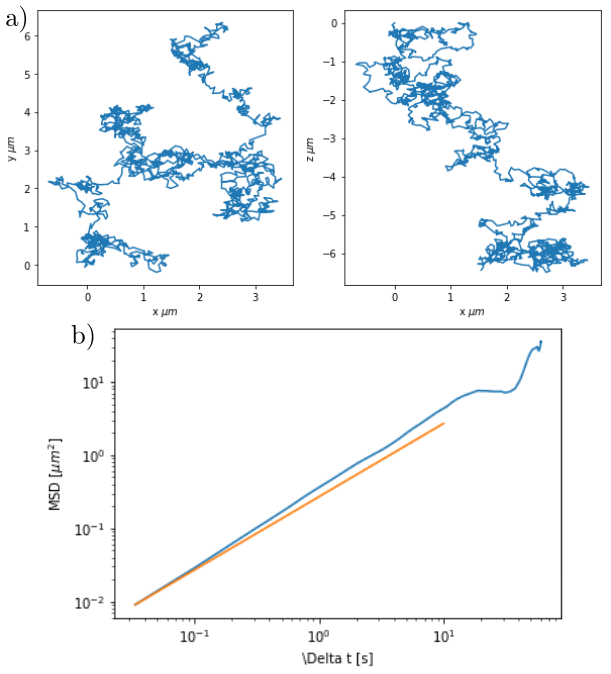
\includegraphics[width=0.8\textwidth]{figures/passivebrowniantrajectorymsd.png}
  \end{center}
  \caption[Example of brownian motion]{A colloidal particle undergoes random, thermally induced displacements in a fluid medium. \textbf{Panel a)} shows the trajectory of the particle. \textbf{ Panel b)} shows the corresponding mean squared displacement (MSD) as a function of time, illustrating the linear relationship predicted by Einstein for diffusive behavior (orange) and the one obtained through a numerical simulation (blue).}\label{fig:passivebrowniantrajectory}
\end{figure}

\section{Directed Motion and the Feynman Ratchet}

The inherent randomness of Brownian motion naturally leads to the question: can this disorder be transformed into order? In other words, can the random thermal motion of particles be used to produce directed movement or extract work? This question sits at the core of statistical mechanics and was famously explored by Richard Feynman in his lectures on physics, through a thought experiment known as the Feynman ratchet and pawl \cite{feynman1963feynman}.

The Feynman ratchet consists of a set of vanes connected to a ratchet wheel, immersed in a fluid (Fig. \ref{fig:feynmanratchet}). The idea is: random collisions from the surrounding molecules could push the vanes, but the pawl only allows rotation in one direction. At first glance, this asymmetric mechanism seems capable of converting random thermal motion into unidirectional rotation, apparently violating the second law of thermodynamics.

\begin{figure}
  \begin{center}
    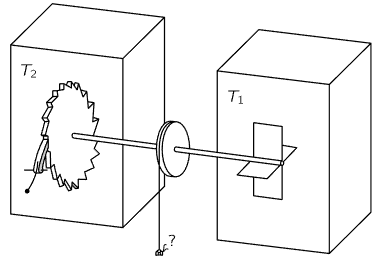
\includegraphics[width=0.65\textwidth]{figures/feynmanratchet.png}
  \end{center}
  \caption[Feynman ratchet]{Visual representation of the Feynman ratchet. Obtained from \cite{feynman1963feynman}}\label{fig:feynmanratchet}
\end{figure}


However, Feynman's analysis showed that when both the ratchet and the pawl are in thermal equilibrium with the same heat bath, the system cannot produce net work. The pawl itself undergoes thermal fluctuations and can occasionally lift off, allowing the ratchet to move backward. Over time, the forward and backward movements average out, and no net rotation occurs. This result reinforces the principle that thermal fluctuations alone cannot be rectified to perform work without a temperature gradient or an external energy input.

Despite this limitation, the Feynman ratchet introduced a powerful concept: asymmetry combined with non-equilibrium conditions can, in principle, produce directed motion. This idea is foundational in the study of Brownian motors, biomolecular machines, and active matter systems, including the systems explored in this thesis. In such systems, energy is continuously supplied, whether through bacterial metabolism or magnetic field modulation, creating the necessary non-equilibrium environment that allows motion rectification to occur.

\chapter{Active and Passive Matter Systems}
\label{ch:activeandpassivemattersystems}

\section{Active matter}

In the study of motion at small scales, materials are often categorized as either active or passive. This distinction is based on whether the constituents are capable of autonomously converting energy into motion.

Active matter refers to systems composed of self-driven units that continuously consume energy to propel themselves \cite{marchetti2013hydrodynamics, bechinger2016active}. Examples include motile bacteria, synthetic Janus particles, and active colloids powered by chemical reactions or light. These systems are inherently out of equilibrium and can exhibit emergent behaviors such as swarming, flocking, and directed transport — even in the absence of external fields.

In contrast, passive matter consists of particles that do not self-propel. Any motion they undergo results from external forces or environmental fluctuations, such as thermal noise or applied fields. Classical Brownian particles are a well-known example of passive matter. However, recent studies have shown that when passive particles are driven by time-asymmetric external fields (e.g., oscillating magnetic fields), they can exhibit behaviors that mimic those of active systems.

This thesis focuses on such externally driven passive systems, particularly on paramagnetic colloids subjected to dynamic magnetic fields. These systems provide a controlled platform to study non-equilibrium transport and rectified motion, drawing inspiration from active matter while remaining fundamentally passive in nature.

\chapter{Motion Rectification in Physical Systems}
\label{ch:motionrectificationinphysicalsystems}

\section{Rectified Motion in Active Matter Systems}

Active matter refers to systems composed of individual units that consume energy to produce motion. These systems inherently operate far from equilibrium and can display collective behaviors such as swarming, clustering, and directed transport. Biological examples include motile bacteria like E. coli, while synthetic realizations include Janus particles and light-activated swimmers. A key feature of active matter is that it can interact with asymmetric boundaries to generate directional motion — a phenomenon central to the idea of active ratchets.

In bacterial systems, for example, interactions with sawtooth-shaped walls can bias the random swimming of cells, leading to net transport or torque on nearby objects. Such rectification has inspired the design of microgears and channels that harness the mechanical output of bacterial baths. Although these systems are active by nature, the underlying mechanism — breaking spatial and temporal symmetry — can also be replicated in driven passive systems.


\section{Driven Motion in Passive Colloidal Systems}

%This physical constraint fundamentally shapes how microorganisms swim and how artificial microswimmers must be designed. Subsequent work by Lauga and Powers [Lauga Powers, 2009] expanded on Purcell's insights by examining the fluid dynamics of various propulsion mechanisms, including bacterial run-and-tumble behavior and the synchronization of flagella. These concepts are directly relevant to systems explored in this thesis, where both biological and magnetically driven entities are used to induce motion in passive structures at the microscale.



\newpage
